\begin{figure}[htbp]
\section*{ ZSWIM6}
\centering
\begin{subfigure}[b]{0.95\textwidth}
\centering
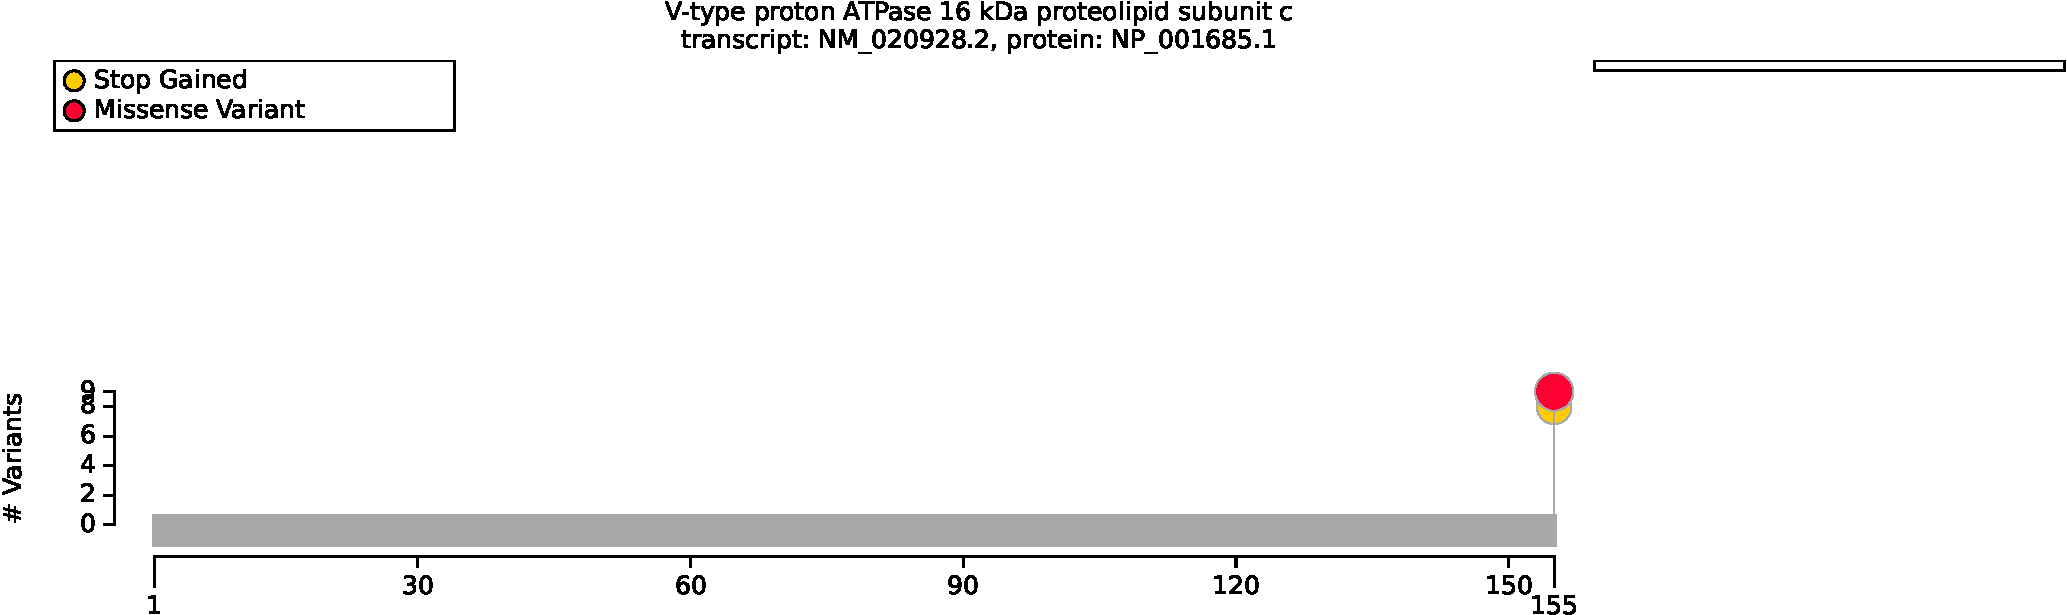
\includegraphics[width=\textwidth]{ img/ZSWIM6_protein_diagram.pdf} 
\captionsetup{justification=raggedright,singlelinecheck=false}
\caption{Distribution of variants in ZSWIM6}
\end{subfigure}

\vspace{2em}

\begin{subfigure}[b]{0.95\textwidth}
\centering
\resizebox{\textwidth}{!}{
\begin{tabular}{llllrr}
\toprule
Genotype (A) & Genotype (B) & total tests performed & significant results\\
\midrule
p.Arg913Ter & Arg1163Trp & 12 & 0\\
\bottomrule
\end{tabular}
}
\captionsetup{justification=raggedright,singlelinecheck=false}
\caption{Fisher Exact Test performed to compare HPO annotation frequency with respect to genotypes.}
\end{subfigure}

\vspace{2em}

\caption{The cohort comprised 16 individuals (8 females, 8 males). A total of 85 HPO terms were used to annotate the cohort. 
Disease diagnoses: Acromelic frontonasal dysostosis (OMIM:603671) (9 individuals), 
Neurodevelopmental disorder with movement abnormalities, abnormal gait, and autistic features (OMIM:617865) (7 individuals). 
No statistically significant results identified. A total of 2 unique variant alleles were found in \textit{ZSWIM6} 
(transcript: \texttt{NM\_020928.2}, protein id: \texttt{NP\_001685.1}).}
\end{figure}
